% Activate the following line by filling in the right side. If for example the name of the root file is Main.tex, write
% "...root = Main.tex" if the chapter file is in the same directory, and "...root = ../Main.tex" if the chapter is in a subdirectory.
 
%!TEX root =  

\chapter{Planning Phase}
\label{plan}

\minitoc 

\subsection*{Purpose}
This chapter details the planning process that seeks to identify the different phases in the development process and allocate resources over time to the various activities that comprise each phase. Planning also needs to account for a number of risk factors that may impact the process, either by allowing for enough preventive measures or by allocating extra time to activities that may be affected. Thus a risk report enumerating several potential risks has been worked out.

\section{Project Phases}\label{phases}
The choice of development model is detailed in Chapter \ref{prelim}. Here the various phases of the project are described.

\subsection{Preliminary Study and Research}
In this phase the aim is for each project member to acquire a certain level domain knowledge in the field of Internet privacy and to learn the necessary technology and tools required to implement the model as proposed by the customer. This entails having a working knowledge of the Java programming language, version control using Git and the CBR framework.

\subsection{Planning}
Planning seeks to identify the activities needed to reach the project objective. This entails breaking down the objectives into sub-problems, identifying the relationship between these, and allocating time for each of them. 

\subsection{Requirement Specification}
The requirements specification is a document listing the functional and non-functional requirements of the software to be developed, which is a standard that the results is to be measured against, thus serving as not only a contract between the customer and the project team, but as a basis for developing testing methods.

\subsection{Design/Architecture}
This phase consists of a broad structuring and specification of the overall system. It defines the program structure in terms of program flow, modules, classes and interfaces as well as coding standards and other conventions that will serve as guidelines for the implementation phase.

\subsection{Implementation}
In this phase the design is realized as a working Java program according to the models developed in the Design phase. 

\subsection{Evaluation and Documentation}
This phase consists of testing the system and documenting the structure of the system and how it is operated. From a software engineering perspective, the primary testing grounds are against the standards prescribed by the requirements specification rather than applicability of the applicability of the CBR agent model to privacy enhancement. As mentioned, among the primary objectives of the project is to provide a testing framework to verify the applicability of the given system in making privacy decisions.

\subsection{Ongoing Activities}

\subsubsection{Reporting and Administrative Tasks}
Under this heading are more project management related activities, such as routine organizational work (ie. arranging meetings and writing status updates), more refined distribution of tasks as the project is underway, and preparation of the project report (this document).

\subsubsection{Study and Lectures}
To solve several of the problems posed by this project, most group members have had to learn new tools and technologies. This includes, but is not limited to Case Based Reasoning, version control (Git), certain features of Java and so on. Lectures on project management  and software development are also subsumed under this heading.

\section{Risk Report}\label{riskReport}
The term \emph{risk} is usually defined as the possibility of an undesirable outcome (loss) as a consequence of a choice or an action made. 


\subsection{Overview and Risk Management}
In this section we have identified some risk factors that can impact the project. Every project does risk management at some level, wether explicit stated or not. By identifying and quantifying the \emph{likelihood} and \emph{consequence} of undesirable events, the project plan can be adapted so as to allow for certain contingencies. Risks are quantified in two dimensions on a scale from 1-5 in severity, both in terms of the probability of occurrence and in terms of the consequence for the project.

The table below contains a sample risk table depicting how risks are described, quantified and which actions are taken to mitigate the particular risk. 


\begin{table}[htdp]
\begin{center}
\begin{tabularx}{\textwidth}{| X | X |}
\hline
\textbf{Risk item} & An arbitrary number identifying the risk factor. \\
\hline
\textbf{Activity} & The activity affected by this risk. \\
\hline
\textbf{Risk Factor} & A short textual description of the risk factor. \\
\hline
\textbf{Probability} & The probability of the event occurring. Measured on a scale from 1(unlikely) to 5(almost certain).\\
\hline
\textbf{Consequence} & What the consequences of the event occurring. Measured on a scale from 1(not critical) to 5(disastrous).\\
\hline
\textbf{Risk} & Probability * Consequence\\
\hline
\textbf{Action taken} & Actions that can be taken to avoid this\\ & event occurring. \\
\hline
\textbf{Deadline} & An optional date set for taking precautions to deal with the risk. \\
\hline
\textbf{Responsible} & The group member responsible for the risk. \\
\hline
\end{tabularx}
\caption{Risk characterization.}
\end{center}
\label{riskTable}
\end{table}



\subsection{Discussion}

As shown in Appendix \ref{riskAppendix}, three broad risk categories were identified:

\begin{enumerate}
\item \textbf{Technical}: These risks pertain mainly to the  implementation; that critical success factors are not met by the implemented software.
\item \textbf{Communication}: These are risks related to miscommunication, either within the project team or between the customer and the team.
\item \textbf{Planning}: The final category has to do with planning and decisions made early on in the project phase.
\end{enumerate}

Among the more critical risks identified were a potential failure to
correctly parse policy documents as well as the risk of an improper
choice of algorithms. Failure to properly parse P3P policies could
impact progress as it would slow down and push the testing phase back
in time. This will also impact the second risk factor above, as an
early testing would reveal the weaknesses of algorithms in time.

An important issue to remedy these problems is a modular design, that
is that these two pieces of functionality are to be isolated in
separate code modules. This implies that if the initial choice of algorithms
made by the project team, while important, are not critical, as they
can be replaced during later development stages.

Other risk factors identified include database and data storage
issues, in particular pertaining to the collaborative filetering
system, and disagreements within the project team. A full listing
of the risk factors identified, and proposed measures to mitigate
these is given in Appendix~\ref{riskAppendix}.


\section{Measurement of project effects}
The primary objective of this project is to build a research prototype that allows for parsing P3P policies and provide advice using CBR given a particular knowledge base. The advice is based on: 

\begin{itemize}
\item the user's previous actions.
\item community actions or what similar users have done.
\item context of use.
\end{itemize}
   

\section{Project Plan}
As discussed in Section~\ref{phases}, the sequential part of the project is separated into six phases; pre-implementation research, requirement specification, design, implementation and documentation, evaluation, and report writing. The reporting started at the first day of the project and continues until project completion. 

Implementation is scheduled to be complete at the end of week 42, which marks a shifting of focus to testing and evaluation. The project plan was initially laid out based on \emph{evidence based scheduling}, starting out with rough estimates of each particular task pertaining to each of the project phases. 

The different components of the system were identified early in the process, and each componentsuch as core CBR and algorithms, networking, GUI and so forth were assigned as the responsibility of a team member. The responsible for each component then provides an estimate over the required time to design, implement and document the component. These estimates will in turn be based on a breakdown of the required tasks for each system. These numbers are then aggregated to form the total plan.

\subsection{Project Milestones}

In the initial plan, four important milestones were laid down to provide a clear measure of progress. The milestones concern the key project phases related to designing, implementing and documenting the system.

\begin{enumerate}
\item \textbf{Requirements specification}: September 21 (Week 38).
\item \textbf{Design}: September 28 (Week 39).
\item \textbf{Implementation and documentation}: October 19 (Week 42).
\item \textbf{Testing and evaluation}: November 2 (Week 44).
\end{enumerate}

A short span between the completion of the requirements specification and the design phases was set as these phases were deemed to be largely overlapping. Many requirements were deemed to be clear from the outset and could therefore be passed on to the design phase without waiting for the formal recognition by the customer. This improves project flow as several key activities occur at the same time.

Similar considerations were made with regard to the implementation and testing milestones. The preparatory steps for the testing work can be conducted in parallell with implementation.

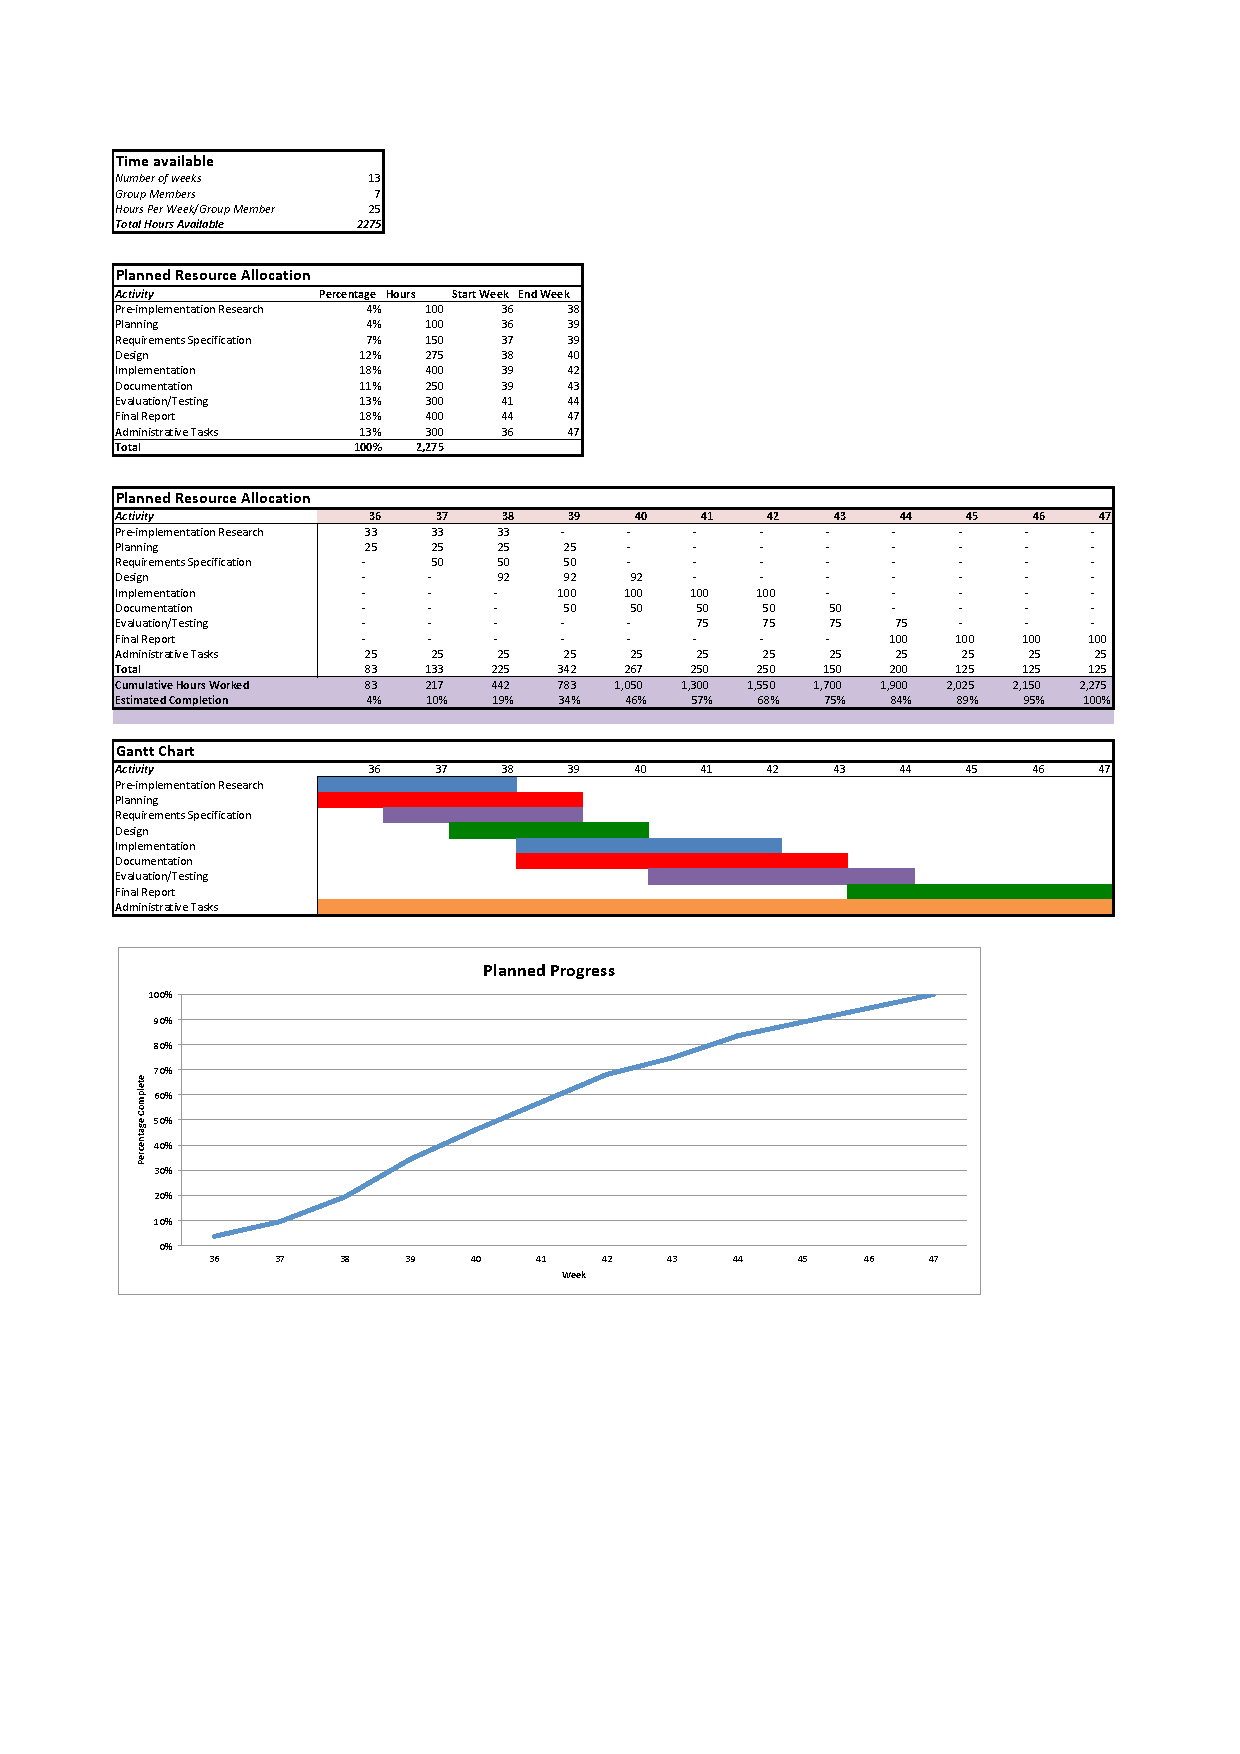
\includepdf{PlanReport/DetailedPlan}
